\section{Workflow}

\subsection{Strong and Weak User Pairs}

The preprocessing of the social networks creates two fast searchable databases for content and structure.  It consists of the following steps:

\begin{enumerate}
	\item obtain the stream of data from the social network
	\item index the twits in a text search engine (Lucene)
	\item build the communication graph (Berkeley DB)
\end{enumerate}

The preprocessing is illustrated in Figure~\ref{figure:preprocessing}.  Note that the term ``preprocessing'' here does not preclude online operation -- the data stream can be indexed continuously, and both Lucene and Berkeley DB allow for efficient real-time growth.

\begin{figure}[htp]
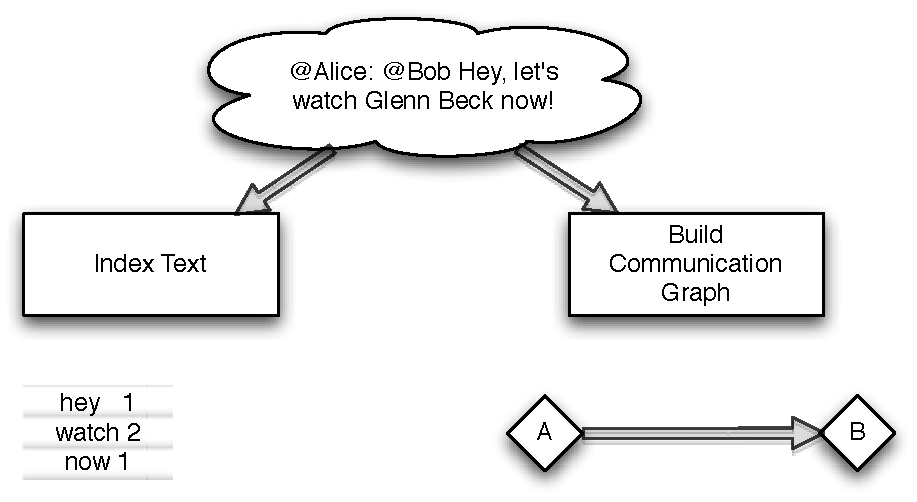
\includegraphics{figures/spie-preprocessing}
\caption{Preprocessing social network data for exploration.  Message text is indexed in a full text search index, and the communication graph is stored in a fast associative map database.}
\label{figure:preprocessing}
\end{figure}


Once those are built, the community sensing workflow proceeds as follows:

\begin{enumerate}
	\item come up with a set of keywords to occur in the community of interest
	\item a seeding pair of repliers about the topic is found
	\item a community of replier triangles is grown from the pair
	\item the characteristic phrases are found for the community discourse
	\item the fringe of the community is identified, with the choices of pairs or topics for further iterations
\end{enumerate}

The exploration workflow is shown in Figure~\ref{figure:workflow}.  

\begin{figure}[htp]
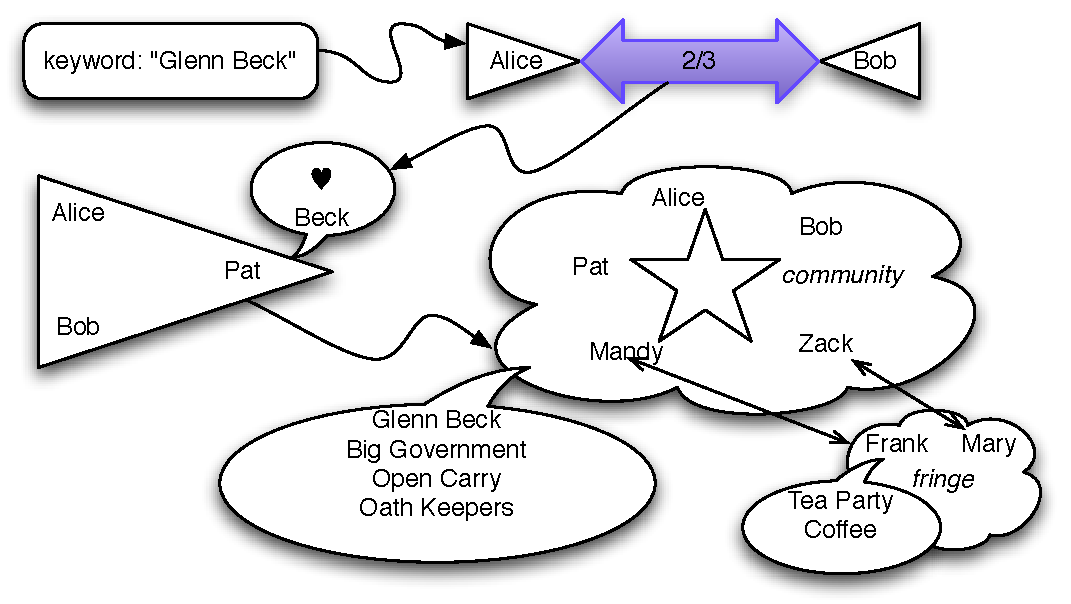
\includegraphics{figures/spie-workflow}
\caption{Exploration workflow.  A keyword is searched and the pairs using it most are found.  Then a community is grown around such a pair, and its topics are extracted.  The fringe and its topics are also listed, allowing for subsequent pivoting and iteration.}
\label{figure:workflow}
\end{figure}
	
\subsection{Finding Topics}

We begin the analysis by searching the Lucene index for pairs of users who discuss a keyword.  All of the twit contents are indexed.  Various twit fields are treated separately, which allows us to find any replies quickly.

\subsection{Finding Communications}

We explored finding both weak and strong pairs of users.  A weak user pair is a pair of users who at least once in their corpora use the same keyword in at least one of their twits and additionally have at least one directed message between them.  A strong pair of users has at least one directed message between them which uses the keyword being searched for.  For our analysis we used strong user pairs finding that they gave us results more like what we were attempting to find as a community.  Additionally, before generating communities based on these pairs we pruned them based on the number of times that the keyword was mentioned between the users.

\subsection{Growing Communities}

We then used these user pairs as seeds for growing communities.  We use a recursive community definition based on a triangle property, such that a user is a member of a community if they have been sent messages by two of the users of the community.  If that is the case, the ``child'' user is added to the community connected to those two ``parent'' users. The child users are added recursively, until there are no more users to add.  Any users which have been sent messages by exactly one of the members of the community is considered to be on the ``fringe'' outside of the community, or simply the fringe.

\subsection{Finding Collocations and SIPs}

We perform collocation and Statistically Improbable Phrase (SIP) analysis on these communities to find the resulting topics of conversation in the communities.  These Natural Language Processing (NLP) approaches are used to identify the most characteristic phrases describing the community discourse, approximating ``what are they talking about.''
